\documentclass[11pt]{article}

% ---------- Packages ----------
\usepackage[margin=1in]{geometry}
\usepackage{amsmath,amsthm,graphicx,enumitem,amssymb}
\usepackage{mathtools}
\usepackage{physics}        % derivatives, bras/kets, etc.
\usepackage{siunitx}        % units
\usepackage{graphicx}       % figures
\usepackage{float}          % figure placement
\usepackage{booktabs}       % nice tables
\usepackage{enumitem}       % better lists
\usepackage{fancyhdr}       % header/footer
\usepackage{titlesec}       % section formatting
\usepackage{hyperref}       % links
\usepackage{tcolorbox}      % boxes for answers
\usepackage{listings}       % code (MATLAB, Python, etc.)
\usepackage{xcolor}
\usepackage{bbm}        % blackboard bold italic

% Define colors
\definecolor{codegreen}{rgb}{0,0.6,0}
\definecolor{codepurple}{rgb}{0.58,0,0.82}
\definecolor{backcolour}{rgb}{0.95,0.95,0.92}

% ---------- Hyperref Setup ----------
\hypersetup{
    colorlinks=true,
    linkcolor=blue,
    urlcolor=blue,
    citecolor=blue
}

% ---------- Header/Footer ----------
\pagestyle{fancy}
\fancyhf{}
\lhead{\textbf{\course}}
\rhead{\textbf{\assignment}}
\cfoot{\thepage}

% ---------- Custom Commands ----------
\newcommand{\course}{ASEN 5264 - DMU}
\newcommand{\assignment}{Homework \#4}
\newcommand{\studentname}{Bijan Jourabchi}

\newcommand{\R}{\mathbb{R}}
\newcommand{\E}{\mathbb{E}}
\newcommand{\Var}{\mathrm{Var}}
\newcommand{\Cov}{\mathrm{Cov}}

% Boxed answer environment
\newtcolorbox{answerbox}{
    colback=gray!5,
    colframe=gray!50,
    title=Answer,
    fonttitle=\bfseries
}

% Problem section format
\titleformat{\section}{\large\bfseries}{Problem \thesection:}{0.5em}{}

% ---------- Code Style ----------
\lstset{
    basicstyle=\ttfamily\small,
    keywordstyle=\color{blue},
    commentstyle=\color{green!50!black},
    stringstyle=\color{orange},
    breaklines=true,
    frame=single
    extendedchars=true,
    literate={π}{{$\pi$}}1 {γ}{{$\gamma$}}1 {α}{{$\alpha$}}1 {ϵ}{{$\epsilon$}}1 {λ}{{$\lambda$}}1 {δ}{{$\delta$}}1
}

% ---------- Document ----------
\begin{document}

% ---------- Title Block ----------
\begin{center}
    {\LARGE \textbf{\course}} \\[6pt]
    {\Large \assignment} \\[10pt]
    \studentname \\
\end{center}

\vspace{1em}
\hrule
\vspace{1em}

% Define Julia language manually
\lstdefinelanguage{Julia}{
  keywords={abstract, break, case, catch, const, continue, do, else, elseif,
      end, export, false, for, function, global, if, import, in, let, local,
      macro, module, otherwise, quote, return, struct, switch, true, try,
      type, typealias, using, while, mutable},
  keywordstyle=\color{blue}\bfseries,
  comment=[l]{\#},
  morecomment=[n]{\#=}{=\#},
  commentstyle=\color{codegreen}\ttfamily,
  stringstyle=\color{codepurple}\ttfamily,
  morestring=[b]',
  morestring=[b]"
}

% General Listing Settings
\lstset{
    language=Julia,
    backgroundcolor=\color{backcolour},   
    basicstyle=\ttfamily\small,
    breaklines=true,                 
    numbers=left,                    
    numbersep=5pt,                  
    frame=single
}

% =====================================================
\section{}

\begin{enumerate}[label=\alph*)]
    \item 
        After a large number of pulls, it is reasonable to assume that $\rho_a \to \theta_a$. However, since we are using an $\epsilon$-greedy
        policy, we still choose randomly with probability $\epsilon$. With probability $1-\epsilon$ we will choose greedily, always picking arm 3. With $\epsilon = 0.15$, we can solve for the probability of pulling arm $a$.
        \begin{align*}
            P(a_1) = \epsilon/3 = 0.05 \\
            P(a_2) = \epsilon/3 = 0.05 \\
            P(a_3) = \epsilon/3 + 1 - \epsilon = 0.9
        \end{align*}

        The expected payoff per pull is given as $\mathbb{E}[R]$, where $\mathbb{E}[R]$ is given by:
        \begin{align*}
            \mathbb{E}[R] = \sum_{k=1}^{3} P(R_i)P(a_i) = 0.2*0.05+0.3*0.05+0.7*0.9 = \boxed{0.655}
        \end{align*}
    \item 
        Again, after a large number of pulls, we have $\rho_a \to \theta_a$. A softmax policy tells us $P(a_3) \propto e^{\lambda\rho_3} = e^{5\theta_3}$.
        In order to obtain a valid probability, we must multiply by a normalizing constant $\frac{1}{c}$ where $c = \sum_{k=1}^{3}e^{5\theta_k}$.
        \begin{align*}
            P(a_3) = \frac{e^{5\theta_3}}{\sum_{k=1}^{3}e^{5\theta_k}} = \frac{33.11}{40.32} = \boxed{0.821}
        \end{align*} 
    \item
        Starting with a prior distribution Beta$(1,1)$, we update the distribution for each arm with Beta$(1+w,1+l)$ where $w$ and $l$ are the total number of wins and losses respectively. For each arm we have the following beliefs.

        \begin{figure}[H]
            \centering
            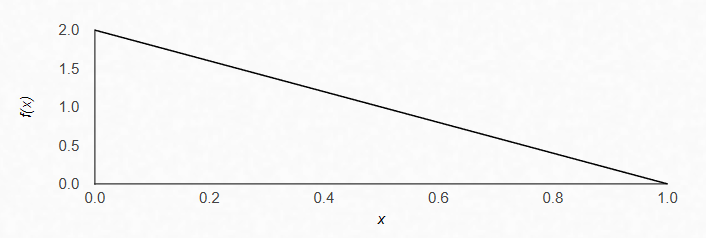
\includegraphics[width=\textwidth, height=0.75\textheight, keepaspectratio]{Beta12.png}
            \caption{Belief for arm 1}
        \label{fig:A1}
        \end{figure}
                \begin{figure}[H]
            \centering
            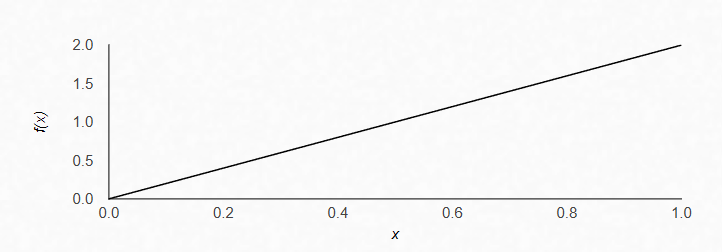
\includegraphics[width=\textwidth, height=0.75\textheight, keepaspectratio]{Beta21.png}
            \caption{Belief for arm 2}
        \label{fig:A2}
        \end{figure}
        \begin{figure}[H]
            \centering
            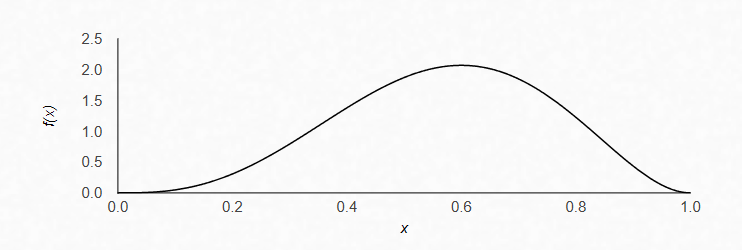
\includegraphics[width=\textwidth, height=0.75\textheight, keepaspectratio]{Beta43.png}
            \caption{Belief for arm 3}
        \label{fig:A3}
        \end{figure}
        \newpage    
    \item
    
    First, we would sample a value $\hat{\theta}_a$ from each belief distribution, then we would choose the arm which had the largest $\hat{\theta}_a$, that is $\arg\max_a \hat{\theta}_a$.
        Some theoretical values that could be sampled are $\hat{\theta}_1 = 0.1$, $\hat{\theta}_2 = 0.8$, $\hat{\theta}_3 = 0.65$. In this case, Thompson sampling would choose arm 2, observe the outcome and update the belief for arm 2.  
\end{enumerate}




% =====================================================
\section{}
Given a policy parameterized with $\theta = [\theta_L,\theta_R]$, we can take the logarithm of the policy, 
$\log(\pi_\theta(s\mid a))$ giving us,

\begin{align*}
    \log(\pi_\theta(a \mid s)) &= \log(\frac{e^{\theta_a}}{e^{\theta_L}+e^{\theta_R}}) = \log(e^{\theta_a}) - \log(e^{\theta_L}+e^{\theta_R}) \\
    \log(\pi_\theta(a \mid s)) &= \theta_a - \log(e^{\theta_L}+e^{\theta_R})
\end{align*}
Using this expression, we can calculate the policy gradients for the given trajectories.
\begin{enumerate}[label =\alph*)]
    \item
    Given $\tau = (1,L,10,2)$, the log policy is \(\log(\pi_\theta(L \mid 1)) = \theta_L - \log(e^{\theta_L}+e^{\theta_R})\). The gradient of the log policy
    is $\nabla_\theta \log(\pi_\theta(L \mid 1))$ where $\nabla_\theta = [\frac{\partial}{\partial \theta_L} \ \ \frac{\partial}{\partial \theta_R}]^T$. Evaluating the gradient at $\theta = [0.5, 0.5]$ we get
    \begin{align*}
        \eval[\frac{\partial \log(\pi_\theta(L \mid 1))}{\partial \theta_L}|_{0.5,0.5} &= \eval[1 - \frac{e^{\theta_L}}{e^{\theta_L} + e^{\theta_R}}|_{0.5,0.5} = 1-\frac{e^{0.5}}{2e^{0.5}} = \frac{1}{2} \\
        \eval[\frac{\partial \log(\pi_\theta(L \mid 1))}{\partial \theta_R}|_{0.5,0.5} &= \eval[ - \frac{e^{\theta_R}}{e^{\theta_L} + e^{\theta_R}}|_{0.5,0.5} = -\frac{e^{0.5}}{2e^{0.5}} = -\frac{1}{2}
    \end{align*}
    Thus,
    \begin{align*}
        \nabla_\theta \log(\pi_\theta (a \mid s)) = \boxed{\begin{bmatrix}
            1/2 \\ -1/2
        \end{bmatrix}}
    \end{align*}
    \item
    Given $\tau = (1,R,20,2)$, the log policy becomes \(\log(\pi_\theta(R \mid 1)) = \theta_R - \log(e^{\theta_L}+e^{\theta_R})\).
    \begin{align*}
        \eval[\frac{\partial \log(\pi_\theta(R \mid 1))}{\partial \theta_L}|_{0.5,0.5} &= \eval[ - \frac{e^{\theta_R}}{e^{\theta_L} + e^{\theta_R}}|_{0.5,0.5} = -\frac{e^{0.5}}{2e^{0.5}} = -\frac{1}{2} \\
        \eval[\frac{\partial \log(\pi_\theta(R \mid 1))}{\partial \theta_R}|_{0.5,0.5} &= \eval[1 - \frac{e^{\theta_R}}{e^{\theta_L} + e^{\theta_R}}|_{0.5,0.5} = 1-\frac{e^{0.5}}{2e^{0.5}} = \frac{1}{2}
    \end{align*}
    Thus,
    \begin{align*}
        \nabla_\theta \log(\pi_\theta (a \mid s)) = \boxed{\begin{bmatrix}
            -1/2 \\ 1/2
        \end{bmatrix}}
    \end{align*}
\end{enumerate}
\newpage
\section{}
Using Flux.jl to fit a neural network to approximate the function $f(x) = (1-x)\sin(20\log(x+0.2))$, I got the results seen in figure \ref{fig:NN}.
\begin{figure}[H]
    \centering
    
\includegraphics[width=\textwidth, height=0.75\textheight, keepaspectratio]{NN_Fxn_Approx.png}
    \caption{Neural Network Function Approximation}
\label{fig:NN}
\end{figure}
\subsection{Code For Problem 3}
\begin{lstlisting}
    using Flux
using Flux.Losses: mse
using Plots
using Statistics: mean
using Plots.PlotMeasures: mm
using ProgressMeter
using Random

f = x -> (1 - x) * sin(20 * log(x + 0.2))
#f = x -> sin(x)

function make_training_data(f)
    x = collect(range(0,1,length=35))
    vcat(x, 0.001)
    y = f.(x)
    return x, y
end

function lossfxn(m, x, y)
    return mse(m(x), y)
end

function train(x_data, y_data; learning_rate=1e-3, n_epochs=1_000, save_every=50, minibatch_size=1)
    x_data = ndims(x_data) == 1 ? reshape(Float32.(x_data), 1, :) : Float32.(x_data)
    y_data = ndims(y_data) == 1 ? reshape(Float32.(y_data), 1, :) : Float32.(y_data)
    @assert size(x_data, 2) == size(y_data, 2) "x_data and y_data must have the same number of samples"
    @assert minibatch_size >= 1 "minibatch_size must be >= 1"

    model = Chain(
        Dense(1=>32, tanh),
        Dense(32=>64, tanh),
        Dense(64=>32, tanh),
        Dense(32=>1)
    )
    opt_state = Flux.setup(Adam(learning_rate), model)

    losses = Float32[]
    models = [deepcopy(model)]


    n_minibatches = Int(length(y_data) / minibatch_size)

    @showprogress for epoch in 1:n_epochs
        batch_loss = zero(Float32)

        for i in 1:n_minibatches
            start_idx = (i - 1) * minibatch_size + 1
            end_idx = i * minibatch_size
            idxs = start_idx:end_idx
            x_minibatch = x_data[:, idxs]
            y_minibatch = y_data[:, idxs]

            function minibatch_objective(model)
                return lossfxn(model, x_minibatch, y_minibatch)
            end

            minibatch_loss, grads = Flux.withgradient(minibatch_objective, model)

            Flux.update!(opt_state, model, grads[1])

            batch_loss += minibatch_loss / n_minibatches
        end

        push!(losses, batch_loss)

        if epoch % save_every == 0
            push!(models, deepcopy(model))
        end
    end

    return models, losses
end

x, y = make_training_data(f)

training_plot = plot(
    vec(x), vec(y),
    label="Training Data",
    xlabel="x",
    ylabel="f(x)",
    title="Training Set",
    linewidth=1.8,
    marker=:circle,
    markersize=2.5,
    color=:navy,
    legend=:topright,
    gridalpha=0.25
)
savefig("training_set.png")

models, losses = train(x, y; learning_rate=5e-4, n_epochs=20_000, minibatch_size=5)

xs = collect(range(0.0f0, 1.0f0, length=100))
truth_vals = f.(xs)
pred_vals = [models[end](Float32[x])[1] for x in xs]

p1 = plot(
    xs, truth_vals,
    label="Truth",
    xlabel="x",
    ylabel="f(x)",
    title="Truth vs NN Approximation",
    linewidth=3,
    color=:steelblue,
    legend=:topleft,
    gridalpha=0.25,
    left_margin=8mm,
    right_margin=4mm,
    top_margin=6mm,
    bottom_margin=8mm
)
scatter!(
    p1, xs, pred_vals,
    label="NN Model",
    color=:tomato,
    markersize=3,
    markerstrokewidth=0,
    alpha=0.85
)

p2 = plot(
    1:length(losses), losses,
    label="Training Loss",
    xlabel="Epoch",
    ylabel="Loss",
    title="Loss vs Number of Epochs",
    linewidth=2.5,
    marker=:circle,
    markersize=3,
    color=:darkgreen,
    legend=:topright,
    gridalpha=0.25,
    left_margin=8mm,
    right_margin=4mm,
    top_margin=6mm,
    bottom_margin=8mm
)

P = plot(
    p1, p2,
    layout=(1, 2),
    size=(1300, 480),
    dpi=150
)

savefig("NN_Fxn_Approx.png") 

\end{lstlisting}
\section{}

The algorithms I chose to implement were Q-Learning and SARSA-$\lambda$. I chose to implement Q-Learning from scratch
since it was essentially the same, if not easier than SARSA-$\lambda$. Q-Learning's main strength is its simplicity and doesn't require tracking eligibility traces like SARSA-$\lambda$.
In addition, Q-Learning is off policy, meaning it learns the optimal policy regardless of the exploration policy. However, the use of $\max$ over the actions leads to maximization bias, causing at times slower learning.
SARSA-$\lambda$ on the other hand is on policy, which can be beneficial in some scenarios. Its main advantage is eligibility traces which allow for temporal credit assignment, meaning we can spread updates backward in time leading to faster convergence.
Generally, Q-Learning has a lower sample complexity compared to SARSA-$\lambda$, and thus it often learns faster in terms of wall clock time. However, this is likely a small difference as they appear to learn just as quickly in figures \ref{fig:Qclk} and \ref{fig:Sclk}.
Despite this, I was able to achieve an average undiscounted reward above 5 with SARSA-$\lambda$ and Q-Learning with little tuning required.
\subsection{Figures}
\begin{figure}[H]
    \centering
    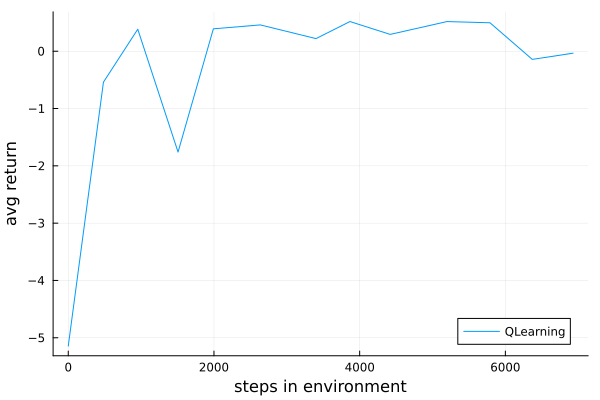
\includegraphics[width=\textwidth, height=0.25\textheight, keepaspectratio]{Q_Steps.png}
    \caption{Q-Learning Average Return vs Steps in Environment}
\label{fig:Qsteps}
\end{figure}

\begin{figure}[H]
    \centering
    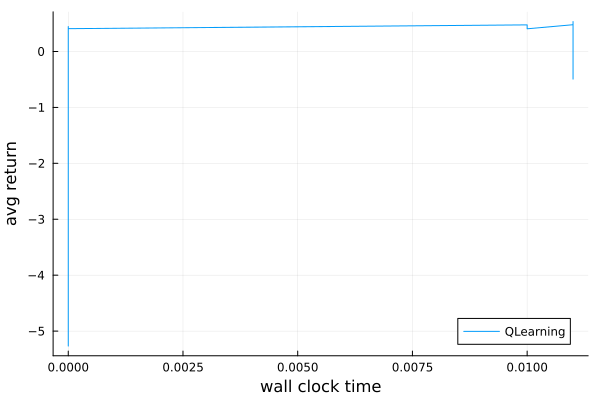
\includegraphics[width=\textwidth, height=0.25\textheight, keepaspectratio]{Q_Clock.png}
    \caption{Q-Learning Average Return vs Wall Clock Time}
\label{fig:Qclk}
\end{figure}

\begin{figure}[H]
    \centering
    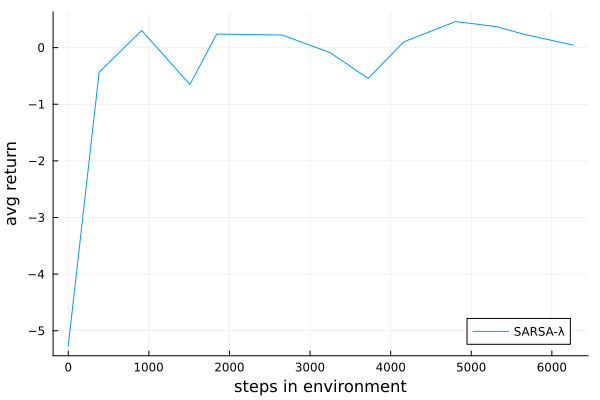
\includegraphics[width=\textwidth, height=0.25\textheight, keepaspectratio]{SARSA_Steps.png}
    \caption{SARSA-$\lambda$ Average Return vs Steps in Environment}
\label{fig:Ssteps}
\end{figure}

\begin{figure}[H]
    \centering
    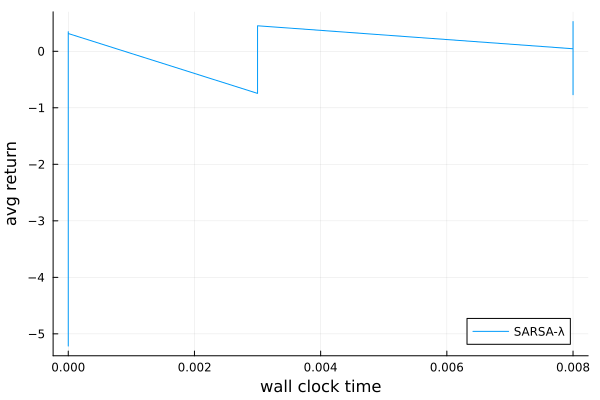
\includegraphics[width=\textwidth, height=0.25\textheight, keepaspectratio]{SARSA_Clock.png}
    \caption{SARSA-$\lambda$ Average Return vs Wall Clock Time}
\label{fig:Sclk}
\end{figure}
\newpage
\subsection{Q-Learning Code}
\begin{lstlisting}
using DMUStudent.HW4: HW4, gw, render
using CommonRLInterface: reset!, actions, act!, observe, terminated, observations
using Plots
using Statistics: mean

function QLearning(env; n_episodes=100000)
    Q = Dict((s, a) => 0.0 for s in observations(env), a in actions(env))
    N = Dict((s, a) => 0.0 for s in observations(env), a in actions(env))
    episodes = []

    for i in 1:n_episodes
        reset!(env)
        push!(episodes, Q_episode(Q,env, N; ϵ=max(0.01, 1-i/n_episodes)))
    end

    return episodes
end

function policy(env, s, ϵ, Q)
    if rand() < ϵ
         return rand(actions(env))
    else
        return argmax(a->Q[(s, a)], actions(env))
    end
end

function evaluate(env, policy; n_episodes=1000, max_steps=1000, γ=1.0)
    returns = Float64[]
    for _ in 1:n_episodes
        t = 0
        r = 0.0
        reset!(env)
        s = observe(env)
        while !terminated(env)
            a = policy(s)
            r += γ^t*act!(env, a)
            s = observe(env)
            t += 1
        end
        push!(returns, r)
    end
    return returns
end

function Q_episode(Q, env, N; ϵ=0.01, γ=0.99, α=0.2)
    start = time()

    s = observe(env)
    hist = [s]
    rhist = []
    while !terminated(env)
        a = policy(env, s, ϵ, Q)
        r = act!(env, a)
        sp = observe(env)

        if terminated(env)
            target = r
        else
            target = r + γ * maximum(ap -> Q[(sp, ap)], actions(env))
        end
        Q[(s,a)] += α * (target - Q[(s,a)])

        s = sp

        push!(hist,sp)
        push!(rhist,r)
    end

    return (hist=hist, rhist=rhist, Q = copy(Q), time=time()-start)
end

episodes = QLearning(gw)


Q = episodes[end].Q
render(gw, policy = s -> argmax(a -> Q[(s,a)], actions(gw)))

function learning_curve_steps(episodes,env)
	p = plot(xlabel="steps in environment", ylabel="avg return")
	n = 40
	stop = 500
	for (name, eps) in episodes
	    Q = Dict((s, a) => 0.0 for s in observations(env), a in actions(env))
	    xs = [0]
	    ys = [mean(evaluate(env, s->argmax(a->Q[(s, a)], actions(env))))]
	    for i in n:n:min(stop, length(eps))
	        newsteps = sum(length(ep.hist) for ep in eps[i-n+1:i])
	        push!(xs, last(xs) + newsteps)
	        Q = eps[i].Q
	        push!(ys, mean(evaluate(env, s->argmax(a->Q[(s, a)], actions(env)), n_episodes=1000)))
	    end    
	    plot!(p, xs, ys, label=name)
	end
	p
end

function learning_curve_clock(episodes,env)
	p = plot(xlabel="wall clock time", ylabel="avg return")
	n = 20 
	stop = 500
	for (name,eps) in episodes
	    Q = Dict((s, a) => 0.0 for s in observations(env), a in actions(env))
	    xs = [0.0]
	    ys = [mean(evaluate(env, s->argmax(a->Q[(s, a)], actions(env))))]
	    for i in n:n:min(stop, length(eps))
	        newtime = sum(ep.time for ep in eps[i-n+1:i])
	        push!(xs, last(xs) + newtime)
	        Q = eps[i].Q
	        push!(ys, mean(evaluate(env, s->argmax(a->Q[(s, a)], actions(env)), n_episodes=1000)))
	    end    
	    plot!(p, xs, ys, label=name)
	end
	p
end

# Associate episodes with a name
Qepisodes = [("QLearning", episodes)]
learning_curve_steps(Qepisodes,gw)
savefig("Q_Steps.png")

learning_curve_clock(Qepisodes,gw)
savefig("Q_Clock.png")

Q_final = episodes[end].Q
policy_final = s -> argmax(a -> Q_final[(s, a)], actions(gw))

returns_undiscounted = evaluate(gw, policy_final; n_episodes=1000, γ=1.0)
avg_undiscounted = mean(returns_undiscounted)

println("Q-Learning Performance Check:")
println("==============================")
println("Average undiscounted cumulative reward: $avg_undiscounted")
println("Requirement: > 5")
println("Success: $(avg_undiscounted > 5 ? "YES" : "NO")")

\end{lstlisting}
\subsection{SARSA-$\lambda$ Code}
\begin{lstlisting}
    using DMUStudent.HW4: HW4, gw, render
using CommonRLInterface: reset!, actions, act!, observe, terminated, observations
using Plots
using Statistics: mean
function sarsa_lambda_episode!(Q, env; ϵ=0.1, γ=0.99, α=0.2, λ=0.99)

    start = time()

    s = observe(env)
    a = rand(actions(env))
    r = act!(env, a)
    sp = observe(env)
    hist = [s]
    N = Dict((s, a) => 0.0)

    function policy(s)
        if rand() < ϵ
            return rand(actions(env))
        end
        return argmax(a -> Q[(s,a)], actions(env))
    end
    

    while !terminated(env)
        ap = policy(sp)

        N[(s, a)] = get(N, (s, a), 0.0) + 1
        
        δ = r + γ*Q[(sp, ap)] - Q[(s, a)]

        for ((s, a), n) in N
            Q[(s, a)] += α*δ*n
            N[(s, a)] *= γ*λ
        end

        s = sp
        a = ap
        r = act!(env, a)
        sp = observe(env)
        push!(hist, sp)
    end

    N[(s, a)] = get(N, (s, a), 0.0) + 1
    δ = r - Q[(s, a)]

    for ((s, a), n) in N
        Q[(s, a)] += α*δ*n
        N[(s, a)] *= γ*λ
    end

    return (hist=hist, Q = copy(Q), time=time()-start)
end
function sarsa_lambda!(env; n_episodes=100, kwargs...)
    Q = Dict((s, a) => 0.0 for s in observations(env), a in actions(env))
    episodes = []
    
    for i in 1:n_episodes
        reset!(env)
        push!(episodes, sarsa_lambda_episode!(Q, env;
                                              ϵ=max(0.01, 1-i/n_episodes),
                                              kwargs...))
    end
    
    return episodes
end
function evaluate(env, policy; n_episodes=50_000, max_steps=1000, γ=1.0)
    returns = Float64[]
    for _ in 1:n_episodes
        t = 0
        r = 0.0
        reset!(env)
        s = observe(env)
        while !terminated(env)
            a = policy(s)
            r += γ^t*act!(env, a)
            s = observe(env)
            t += 1
        end
        push!(returns, r)
    end
    return returns
end

lambda_episodes = sarsa_lambda!(gw, n_episodes=100_000, α=0.05, λ=0.9);
episodes = Dict("SARSA-λ"=>lambda_episodes)


Q = lambda_episodes[end].Q
render(gw, policy = s -> argmax(a -> Q[(s,a)], actions(gw)))

function learning_curve_steps(episodes,env)
	p = plot(xlabel="steps in environment", ylabel="avg return")
	n = 40
	stop = 500
	for (name, eps) in episodes
		  
	    Q = Dict((s, a) => 0.0 for s in observations(env), a in actions(env))
	    xs = [0]
	    ys = [mean(evaluate(env, s->argmax(a->Q[(s, a)], actions(env))))]
	    for i in n:n:min(stop, length(eps))
	        newsteps = sum(length(ep.hist) for ep in eps[i-n+1:i])
	        push!(xs, last(xs) + newsteps)
	        Q = eps[i].Q
	        push!(ys, mean(evaluate(env, s->argmax(a->Q[(s, a)], actions(env)), n_episodes=1000)))
	    end    
	    plot!(p, xs, ys, label=name)
	end
	p
end
learning_curve_steps(episodes,gw)
savefig("SARSA_Steps.png")

function learning_curve_clock(episodes,env)
	p = plot(xlabel="wall clock time", ylabel="avg return")
	n = 20
	stop = 500
	for (name,eps) in episodes
	    Q = Dict((s, a) => 0.0 for s in observations(env), a in actions(env))
	    xs = [0.0]
	    ys = [mean(evaluate(env, s->argmax(a->Q[(s, a)], actions(env))))]
	    for i in n:n:min(stop, length(eps))
	        newtime = sum(ep.time for ep in eps[i-n+1:i])
	        push!(xs, last(xs) + newtime)
	        Q = eps[i].Q
	        push!(ys, mean(evaluate(env, s->argmax(a->Q[(s, a)], actions(env)), n_episodes=1000)))
	    end    
	    plot!(p, xs, ys, label=name)
	end
	p
end
learning_curve_clock(episodes,gw)
savefig("SARSA_Clock.png")



Q_final = lambda_episodes[end].Q
policy_final = s -> argmax(a -> Q_final[(s, a)], actions(gw))

returns_undiscounted = evaluate(gw, policy_final; n_episodes=1000, γ=1.0)
avg_undiscounted = mean(returns_undiscounted)

println("SARSA-Lambda Performance Check:")
println("==============================")
println("Average undiscounted cumulative reward: $avg_undiscounted")
println("Requirement: > 5")
println("Success: $(avg_undiscounted > 5 ? "YES" : "NO")")


\end{lstlisting}
% =====================================================

\end{document}
